\chapter{Environment}
\label{chapter:environment}
This chapter demonstrates few of the different options available for low-level automated testing in Java-projects. First,
\textbf{xUnit testing frameworks} are explained with JUnit as an example of them. Second, \textbf{implementation level BDD testing frameworks}
running on top of JVM programming languages are demonstrated as an alternative for automated low-level Java-code testing.

\section{xUnit testing frameworks} %2p
    xUnit family of testing frameworks are free, open source software for various programming languages that
    all share the same basic architecture. The first implementation of a xUnit test framework was \textit{SUnit}
    for Smalltalk in 1999.  From there the same idea was ported for Java and thus \textit{JUnit} was born. There exists also many other
    xUnit family members, for instance \textit{CppUnit} for C++, \textit{NUnit} for .NET languages and \textit{PyUnit} for Python.
    These unit testing frameworks are extensible with different types of extensions. Extensions can add for example integration testing capabilities
    for different domains. ~\cite{hamill2004unit}

    This thesis is interested in developer practices with JUnit and their perception towards it, therefore next the xUnit family architecture
    is examined with JUnit.

    \subsection{JUnit}
    JUnit acts as the reference implementation of the xUnit family and it is also the most popular instance of them~\cite{hamill2004unit}.
    It is used for Java-code testing and it can be extended for many domains in Java testing~\cite{hamill2004unit}.
    Current stable version of JUnit is \textit{JUnit4}~\cite{junit4}, but \textit{JUnit5} is scheduled to release in Q5 of 2017~\cite{junit5schedule}
    providing many new features for Java testing. The examples of JUnit and empirical research in this thesis are all based on JUnit4.

    \begin{figure}[ht]
      \begin{center}
        \includegraphics[width=13cm]{images/junit.png}
        \caption{JUnit architecture}
        \label{fig:junit}
      \end{center}
    \end{figure}

    The basic architecture close to reference implementation of xUnit testing family~\cite{hamill2004unit} is explained with
    \textit{JUnit3}. The architecture of JUnit3 consists of classes \textit{TestCase, TestRunner, TestFixture, TestSuite} and \textit{TestResult}.
    \textbf{TestCase} is the unit test base class, that holds runnable \textbf{test methods}.
    It implements the interface \textbf{Test} and its \textit{run()}-method. Test methods use \textbf{assertions} inside them to evaluate test conditions.
    \textbf{TestRunner} class is for extending JUnit and running multiple test cases at once and reporting
    them. \textbf{TestFixture} class is used to ensure test isolation and creating a separate test environment for each test method.
    TestFixtures provide a common shared context for test methods, but the environment is created from scratch for each test.
    This is enabled by providing the test case with common setup and teardown functionality for class and method level.
    \textbf{TestSuite} is a class made for grouping TestCases and it also implements Test. TestSuite makes it possible to run multiple TestCases and can
    be used with TestRunner. \textbf{TestResult} class is used to collect test method outcomes from TestSuites and TestCases.
    Figure \ref{fig:junit} visualizes the relationships between the core classes, interfaces and methods of JUnit architecture. ~\cite{hamill2004unit}

    JUnit is a \textit{"Spartan"} test framework, it contains only the mandatory features and has to use additional libraries
    to provide additional testing features such as as mocking or \textbf{Data Driven Testing (DDT)}~\cite{kapelonis2016java}.
    In the next section, example is provided of a JUnit4 test case extended for integration testing of Spring Framework domain.

    \subsection{Extending JUnit for Spring Framework domain}
    \label{section:junit-extend}
    \textbf{Spring} is a framework for Java, described as:
    \textit{"core support for dependency injection, transaction management, web applications, data access, messaging, testing and more."}~\cite{spring}
    It is targeted for Java enterprise applications, providing teams with a framework that allows them to primarily focus on
    application's business logic~\cite{spring}. Spring framework ships with a lot modules and features that needs to be
    configured for the project~\cite{wiki:spring}. \textbf{Spring Boot} is \textit{convention-over-configuration} solution
    composed of the Spring Framework components, that enables rapid application development with minimal effort to get started~\cite{wiki:spring}.

    Spring Framework integration testing can be done by extending JUnit with custom \textit{Spring JUnit runner} class or by using Spring \textit{JUnit class and
    method rules}. Runner class and the Spring JUnit rules both provide standard Spring test context
    for integration tests with features such as dependency injection and transactional test method execution. ~\cite{springintegration}

    \begin{figure}[ht]
        \begin{lstlisting}[style=java]
    %%@RunWith%%(SpringJUnit4ClassRunner.class)
    $$@SpringBootTest
    public class GameServiceIntegrationTest {
        $$@Autowired
        private GameService gameService;

        $$@Autowired
        private GameRepository gameRepository;
        \end{lstlisting}
        \caption{JUnit extended for Spring integration testing}
        \label{fig:springrunner}
    \end{figure}

    Figure \ref{fig:springrunner} shows example of a Spring Boot JUnit integration test, where the \textbf{context and its configuration} are
    loaded with lines 1 and 2. Line \#2 is an example of extending JUnit with custom runner. Lines 4-5 and 7-8 show
    examples of \textbf{injected dependency} via Spring Framework.

    Figure \ref{fig:junit-examples} displays the usage of \textbf{fixture} and two \textbf{test methods}. At lines 4-8 the fixture method
    inits separately before each test method run two common variables used in both tests. Lines 10-11 and 19-20 display two test method definitions with the
    \textit{@Test}-annotation from JUnit4. When used, it marks the following method as a runnable test method. Both test methods
    contain \textbf{assertions}. Assertions in use at lines 14-16 and 26 are \textit{Hamcrest matchers}~\cite{hamcrest}, that
    allows more readable descriptions for used assertions than traditional JUnit assertions.

    \begin{figure}[H]
        \begin{lstlisting}[style=java]
    private GameDifficulty gameDifficulty;
    private String playerName;

    $$@Before
    public void !!initGameValues!!() {
        gameDifficulty = GameDifficulty.NORMAL;
        playerName = "Player";
    }

    $$@Test
    public void !!testStartGameWithNormalDifficulty!!() {
        Game createdGame = gameService.startGame(playerName, gameDifficulty);

        assertThat(createdGame, is(notNullValue()));
        assertThat(createdGame.getPlayerName(), equalTo(playerName));
        assertThat(createdGame.getDifficultyLevel(), equalTo(gameDifficulty));
    }

    $$@Test
    public void !!testStartGamePersistsToDB!!() {
        Integer gameCountBeforeStartGame = gameRepository.findAll().size();

        gameService.startGame(playerName, gameDifficulty);

        Integer gameCountAfterStartGame = gameRepository.findAll().size();
        assertThat(gameCountAfterStartGame, is(greaterThan(gameCountBeforeStartGame)));
    }
        \end{lstlisting}
        \caption{JUnit Spring Framework integration tests}
        \label{fig:junit-examples}
    \end{figure}

    Figure \ref{fig:junit-result} shows the result of the test case run. Even though the example test methods start with the word test,
    JUnit4 allows free format naming of the test methods that don't need to start with test. This also allows to use JUnit as a tool for practicing
    implementation level BDD with some added verbosity in test method naming~\cite{smart2014bdd}.

    \begin{figure}[H]
      \begin{center}
        \begin{topbot}[style=mdstyle]
        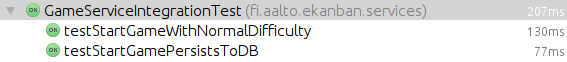
\includegraphics[width=\textwidth]{images/junit-result.png}
        \end{topbot}
        \caption{JUnit test run results}
        \label{fig:junit-result}
      \end{center}
    \end{figure}

    Build configuration of JUnit4 used in examples can be found in Appendix \ref{chapter:gradle-build} figure \ref{fig:junit-build}.
    Used build tool is Groovy-based \textit{Gradle}~\cite{gradle}.
    JUnit and its extensions provide a base for automated low-level testing of Java-code.
    In the next section alternatives for Java-code testing are presented with implementation level BDD testing frameworks from
    various JVM programming languages.

\section{Implementation level BDD testing frameworks for JVM}
    As this thesis is interested in testing Java-code, the scope of implementation level BDD is limited to testing frameworks
    found from JVM programming languages. As stated before, these languages hold ones such as \textit{Ruby, Groovy, Python,
    Clojure} and \textit{Scala}. Through all these languages there exists many alternatives for both implementation and
    acceptance level BDD testing frameworks. For implementation level, there exists two alternative approaches to practicing
    BDD: \textbf{xSpec family}~\cite{solis2011study} and \textbf{Gherkin family} testing frameworks.

    \subsection{xSpec family}
    xSpec family testing frameworks are restricted to implementation level~\cite{solis2011study}. xSpec style testing
    is examined in more detail in this section through \textbf{\textit{RSpec}} via JRuby, but it also demonstrated with
    Java 8 -based \textbf{\textit{Spectrum}}. There exists also other possibilities for xSpec family testing in JVM enviroment,
    one of them being for example Scala-based \textbf{FunSpec}~\cite{funspec} for ScalaTest, but it is not examined in detail.

    \subsubsection{RSpec}
    Ruby community has been for a long time a steady advocate of TDD~\cite{lerner2009forge}. It is also the birth place
    of first implementation level BDD testing framework: RSpec~\cite{astels2006new}. Whereas first BDD framework
    JBehave~\cite{bdd2006north} was aimed for acceptance level and all stakeholders, RSpec brought the behavior driven thinking for developer
    audience~\cite{astels2006new}.

    RSpec is the founding framework in xSpec family of testing. In its current version 3.5, it is a mature holistic testing
    framework including \textit{expectations} library (assertions), \textit{mocking capabilities, integrations} to Ruby frameworks and the \textit{core runner}~\cite{rspecdoc}.
    Later on in this section, RSpec usage for testing Java-code both at unit and integration level for Spring framework is reviewed.
    Before this, the core concepts of RSpec are illustrated.

    The main functionality of RSpec comes from the \textit{rspec-core} library~\cite{rspecdoc}. It includes the code \textbf{example groups} that can hold runnable
    specification \textbf{code examples}~\cite{chelimsky2010rspec}. These examples and groups are created into a \textbf{spec} file~\cite{chelimsky2010rspec}.
    Example groups can be initialized with keywords \textit{describe}
    and \textit{context}, which both are aliases for each other~\cite{rspec-core}. Example groups can inherit each other nested in a single
    file, creating nested context groups~\cite{rspec-core}. This can help immensively on removing
    repetition from the test code
    and achieving easily readable test outputs~\cite{chelimsky2010rspec}. This is enabled by easily usable \textbf{lifecycle hooks},
    such as \textit{before, after} and \textit{around}~\cite{chelimsky2010rspec}.
    These lifecycle hooks can be used to run separately for each example or just once for all examples in the example group.

    Specification code examples can be created with the keywords \textit{it, specify} and \textit{example}~\cite{rspec-core}.
    These examples create executable pieces of behavior of the code under specification~\cite{chelimsky2010rspec}. Code examples
    contain \textbf{expectations}, which specify the expected behavior of the given example~\cite{chelimsky2010rspec}. Expectations can
    be seen as assertions from xUnit testing family, but the reason for changing the language is to support better communication
    between stakeholders, in this case developers~\cite{chelimsky2010rspec}. As BDD is an evolution of TDD, expectations
    was created to establish a better language for what the code to be developed \textit{should} do, instead of verifying it
    with assertions~\cite{astels2006new}. The guideline for the code examples is to hold only one expectation per example~\cite{chelimsky2010rspec}.
    This allows separate info about failing situations~\cite{chelimsky2010rspec} and provides a rule \textbf{one assert per test method}
    for living specification~\cite{astels2006new}. This rule was originally created by Astels~\cite{astels2006new} to
    help TDD practitioners to change viewpoint from 1-1 relationship between test classes and methods to production classes
    and methods.
    The following table shows the relationships between RSpec testing terms compared to xUnit architecture components~\cite{chelimsky2010rspec}:

    \begin{longtable}{@{}p{0.25\textwidth}p{0.7\textwidth}@{}}
    Expectations & $\Longrightarrow$  \textrm{Assertions} \\
    Code Example & $\Longrightarrow$  \textrm{Test Method} \\
    Example Group & $\Longrightarrow$  \textrm{Test Case} \\
    Spec File & $\Longrightarrow$  \textrm{Test Suite} \\
    Lifecycle Hook & $\Longrightarrow$  \textrm{Test Fixture} \\
    \end{longtable}

    \begin{figure}[H]
        \begin{lstlisting}[style=ruby]
    describe !!GameService!! do

      before(%%:all%%) do
        %%@gameInitService%% = !!Mockito!!.mock(!!GameInitService!!.java_class)
        %%@playerService%% = !!Mockito!!.mock(!!PlayerService!!.java_class)
        %%@gameOptionService%% = !!Mockito!!.mock(!!GameOptionService!!.java_class)
        %%@gameRepository%% = !!Mockito!!.mock(!!GameRepository!!.java_class)
        %%@game_service%% = !!GameService!!.new(%%@gameInitService%%, %%@playerService%%,
                                           %%@gameOptionService%%, %%@gameRepository%%)
      end
        \end{lstlisting}
        \caption{RSpec unit test spec file initializing}
        \label{fig:rspec-init}
    \end{figure}

    Figure \ref{fig:rspec-init} displays the creation of a spec file. The spec file example is created for unit testing
    of \textit{GameService} Java-class. Line \#1 shows the creation of example group with the keyword \textit{describe}. Lines from
    3 to 10 show the lifecycle hook \textit{before}, that is used once before all code examples in the example group.
    In the before hook, BDD Gherkin inspired Java mocking library \textbf{Mockito}~\cite{mockito} is used for
    creating test double objects that replace the dependencies of GameService.

    Figure \ref{fig:rspec-example} illustrates use of nested example groups that contains two examples in the second
    level nested example group. Line \#1 is the first example group, that is created with keyword \textit{describe}. The second
    level nested example group starts at line \#9 and it is initialized with the keyword \textit{context}. The \textbf{context} of
    example method is a combined from the lifecycle hooks and variable declarations of the nested example group structure.

    \begin{figure}[H]
        \begin{lstlisting}[style=ruby]
    describe 'startGame()' do
      let(%%:player_name%%) {"Player"}
      let(%%:game_difficulty%%) {!!GameDifficulty::NORMAL!!}
      let(%%:new_game%%) {!!GameBuilder!!.aGame().
                          with_player_name(player_name).
                          with_difficulty_level(game_difficulty).
                          build()}

      context 'with normal difficulty' do

        before(%%:each%%) do
          !!Mockito!!.&&when&&(%%@gameInitService%%.getInitializedGame(
              !!Mockito!!.any(GameDifficulty.java_class), !!Mockito!!.anyString)).thenReturn(new_game)
          !!Mockito!!.&&when&&(%%@gameRepository%%.save(new_game)).thenReturn(new_game)
        end

        subject(%%:created_game%%) { %%@game_service%%.start_game(player_name, game_difficulty) }

        it 'should create game with the given name' do
          expect(created_game.player_name).to eq player_name
        end

        it 'should create game with the given game difficulty' do
          expect(created_game.difficulty_level).to eq game_difficulty
        end

      end
    end
        \end{lstlisting}
        \caption{RSpec nested example groups with code examples}
        \label{fig:rspec-example}
    \end{figure}

    RSpec lets to define the \textbf{action} of the example group with the keyword \textit{subject}~\cite{rspec-subject}. Example of used subject is at
    line 17. The two code examples are at lines 19-21 and 23-25.  Both examples show \textbf{expectations} given with keyword \textit{expect}
    at lines 20 and 24. The two expectations are separated from each other following the \textit{one assert per test method}
    to create more granular documentation of behavior. As mentioned earlier, this separation also allows independently failing code examples.
    \newgeometry{bottom=1cm}
    \begin{figure}[H]
      \begin{center}
        \begin{topbot}[style=mdstyle]
        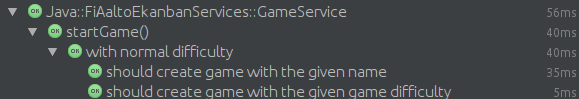
\includegraphics[width=\textwidth]{images/rspec-result.png}
        \end{topbot}
        \caption{RSpec code example run output}
        \label{fig:rspec-result}
      \end{center}
    \end{figure}

    Figure \ref{fig:rspec-result} shows the output of code examples run in Integrated Development Environment (IDE) \textit{Intellij Idea}~\cite{intellij}.
    The nested structure of example groups
    is seen with accordion elements. At the leaf of the nested tree structure is the code example and its run result. In
    reporting, the output of first code example is formatted as
    \begin{center}
    \textit{Java::FiAaltoEkanbanServices::GameService startGame() with normal difficulty should create game with given name}
    \end{center}

    Extending RSpec for Spring Framework domain integration testing needs to be done different route than with JUnit. RSpec
    runner can't use custom JUnit Spring runner or JUnit Spring context rules. Example group also can't be annotated with
    spring configuration. Configuration annotation can be used with other demonstrated testing frameworks in this chapter. Figure \ref{fig:rspec-config}
    displays the configuration that enables Spring Framework context for RSpec testing. At line \#6, it scans the given
    package for dependencies. At lines 7-9 test specific configuration is registered for the test context. Lines 17-19
    display how to retrieve web server port for integration testing.

    \begin{figure}[H]
        \begin{lstlisting}[style=ruby]
    class !!SpringContext!!
      include !!Singleton!!

      def initialize
        %%@ctx%% = !!AnnotationConfigEmbeddedWebApplicationContext!!.new
        %%@ctx%%.scan("fi.aalto.ekanban")
        %%@ctx%%.getEnvironment.setActiveProfiles("test")
        %%@ctx%%.register(!!MongoConfiguration!!.java_class)
        %%@ctx%%.register(!!PortConfiguration!!.java_class)
        %%@ctx%%.refresh
      end

      def spring_ctx
        %%@ctx%%
      end

      def spring_port
        %%@ctx%%.getEmbeddedServletContainer.getPort
      end
    end
        \end{lstlisting}
        \caption{RSpec extension for Spring Framework integration testing}
        \label{fig:rspec-config}
    \end{figure}

    \restoregeometry

    Figure \ref{fig:rspec-autowire}
    illustrates how-to inject dependencies for RSpec integration testing through Spring Framework dependency injection container.
    At line 13 the Spring Framework test context is created and at line 14 additional dependency is retrieved
    through the initialized singleton integration test context object.

    \begin{figure}[ht]
        \begin{lstlisting}[style=ruby]
    describe !!GameService!! do

      before(%%:all%%) do
        %%@ctx%% = !!SpringContext!!.instance.spring_ctx
        %%@gameRepository%% = %%@ctx%%.getBean "gameRepository"
      end
        \end{lstlisting}
        \caption{Spring Framework dependency injection example for RSpec}
        \label{fig:rspec-autowire}

    \end{figure}

    To be included in the build process, getting JRuby-based RSpec in use for testing Java-code needs more setup than
    other testing frameworks reviewed in this chapter. Appendix \ref{chapter:gradle-build} figure \ref{fig:rspec-build}
    displays the full build configuration
    needed to make RSpec a part of a \textit{Gradle} build. To be able to run the tests in IDE \textit{Intellij Idea}},
    JRuby environment with the needed \textit{ruby gems}~\cite{rubygems} (dependencies) installed is required.

    \subsubsection{Spectrum}
    Spectrum is a Java 8 -based BDD-style \textbf{test runner for JUnit4}. It is influenced by BDD implementation
    level testing frameworks \textit{Jasmine} and \textit{RSpec}. It is used via custom runner for JUnit, and thus has good support for
    IDEs and reporting tools that are used with JUnit. Version 1.1.0 of Spectrum supports both xSpec family specification style and Gherkin
    family structure. This thesis inspects Spectrum more closely as a RSpec alternative for xSpec family style testing of Java-code.~\cite{spectrum}

    Spectrum used in examples and later on in projects is version 1.0.2. It supports nested \textbf{example groups} initialized
    with the keyword \textit{describe} and \textbf{code examples} with keyword \textit{it}. Both the example groups and their code
    examples are build with Java 8 lambda blocks. It has also support for \textbf{lifecycle hooks} \textit{before} and \textit{after}. ~\cite{spectrum-102}

    Figure \ref{fig:spectrum-example} displays the exact same Java-based specification as the JRuby RSpec one in figure \ref{fig:rspec-example}.
    The main difference is the added verbosity from Java compared to Ruby. Otherwise the used example groups and their code examples
    match one to one. Exceptions in used terminology are missing keywords \textit{context} and \textit{subject}.
    Deviation from RSpec is also the usage of \textbf{assertions} with \textit{Hamcrest matchers} instead of \textit{expectations}.
    Figure \ref{fig:spectrum-result}
    displays the output of code example runs in IDE Intellij Idea.

    \begin{figure}[H]
    \begin{lstlisting}[style=java]
    describe("startGame", () -> {

        final Supplier<GameDifficulty> gameDifficulty = let(() -> GameDifficulty.NORMAL);
        final Supplier<String> playerName = let(() -> "Player");
        final Supplier<Game> newGame = let(() -> GameBuilder.aGame()
                                                    .withPlayerName(playerName.get())
                                                    .withDifficultyLevel(gameDifficulty.get())
                                                    .build());

        describe("with normal difficulty", () -> {

            beforeEach(() -> {
                Mockito.when(gameInitService.getInitializedGame(
                        Mockito.any(GameDifficulty.class),
                        Mockito.any(String.class))).thenReturn(newGame.get());
                Mockito.when(gameRepository.save(Mockito.any(Game.class))).thenReturn(newGame.get());
            });

            final Supplier<Game> createdGame = let(() ->
                    gameService.startGame(playerName.get(), gameDifficulty.get()));

            it("should create game with the given name", () -> {
                assertThat(createdGame.get().getPlayerName(), equalTo(playerName.get()));
            });

            it("should create game with the given game difficulty", () -> {
                assertThat(createdGame.get().getDifficultyLevel(), equalTo(gameDifficulty.get()));
            });

        });
    });
    \end{lstlisting}
        \caption{Spectrum nested example groups with code examples}
        \label{fig:spectrum-example}

    \end{figure}

    \begin{figure}[H]
      \begin{center}
        \begin{topbot}[style=mdstyle]
        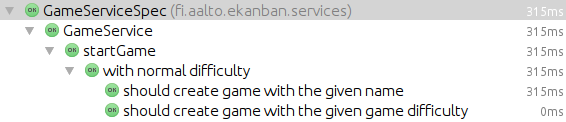
\includegraphics[width=\textwidth]{images/spectrum-result.png}
        \end{topbot}
        \caption{Spectrum code example run output}
        \label{fig:spectrum-result}
      \end{center}
    \end{figure}

    Extending Spectrum 1.0.2 for Spring Framework domain integration testing happens with context configuration and imperative
    creation of test context. At line 21 in Figure \ref{fig:spectrum-init}, JUnit is extended with custom \textit{Spectrum-runner}.
    This enables the usage of example groups and code examples. Line \#2 shows the annotation based configuration of the Spring Boot
    test context. As mentioned in section \ref{section:junit-extend} about extending JUnit for Spring Framework,
    the normal extending for Spring Framework would
    happen with custom \textit{JUnit Spring runner} or \textit{JUnit rules}. Neither of these options work with the Spectrum version in use,
    but line \#13 displays alternative imperative way of loading test context. Lines 5-6 and 8-9 display the dependency
    injection feature of Spring Framework.

    \begin{figure}[H]
    \begin{lstlisting}[style=java]
    %%@RunWith%%(Spectrum.class)
    $$@SpringBootTest
    public class GameServiceIntegrationSpec {

        $$@Autowired
        private GameService gameService;

        $$@Autowired
        private GameRepository  gameRepository;

        {
            beforeAll(() -> {
                new TestContextManager(getClass()).prepareTestInstance(this);
            });
    \end{lstlisting}
        \caption{Spectrum extension for Spring Framework integration testing}
        \label{fig:spectrum-init}
    \end{figure}

    Build configuration for shown examples can be found in Appendix \ref{chapter:gradle-build} figure \ref{fig:spectrum-build}.
    The used build tool is \textit{Gradle}.

    Essentially Spectrum is a Java-based implementation of a \textbf{subset of features present in RSpec}. It is at early version,
    and is not yet mature or widely used framework. Still, it can be considered as a fully working instance of a xSpec family
    testing framework. Next section examines the alternative implementation level BDD testing approach: Gherkin family.


    \subsection{Gherkin family}
    Gherkin family is a term defined in this thesis, containing BDD testing frameworks that use predetermined ubiquitous
    language \textbf{Gherkin}~\cite{gherkin}. There exists research related to usage of Gherkin in BDD testing frameworks~\cite{okolnychyi2016study}.
    Gherkin family frameworks exists for both acceptance and implementation testing level~\cite{okolnychyi2016study}. For Java-code testing at
    implementation level with Gherkin, JVM offers for example \textbf{\textit{Spock}}~\cite{spock} via Groovy, Java 8 -based \textbf{\textit{Spectrum}}~\cite{spectrum},
    JRuby-based \textbf{RSpec-given}~\cite{rspec-given} for Rspec and Scala-based \textbf{FeatureSpec}~\cite{featurespec} for ScalaTest.
    Spock will be used as an example for inspecting implementation level testing with a Gherkin family framework.

    \subsubsection{Spock}
    Spock is a BDD testing framework for JVM programming language Groovy~\cite{kapelonis2016java}. It supports
    testing both Java and Groovy code and it can be considered a superset of JUnit, as it extends the JUnit runner~\cite{spock}.
    As a result of this, it is considered "enterprise ready" with \textit{support for IDEs, JUnit rules, external tools} that use
    JUnit runner and easy \textit{build tool integrations}~\cite{kapelonis2016java}.

    Spock is capable of testing the whole automated BDD cycle from acceptance level to unit level~\cite{kapelonis2016java}.
    It holds unit test support with integrated mocking and stubbing capabilities~\cite{spock}.
    Spock can also be extended for integration testing of different domains~\cite{kapelonis2016java}.
    Spring Framework domain extension is done with \textit{spock-spring} dependency, that can be configured with
    the \textit{@ContextConfiguration}-annotation of Spring~\cite{springintegration}.

    Spock also supports \textbf{DDT} with tabular format readable
    domain specific language (DSL)~\cite{spock}.
    DDT can drastically remove repetition from test code and makes it easier to test different parameter
    variations~\cite{kapelonis2016java}.
    Figure \ref{fig:spock-debug} displays console debugger of Spock related to
    condition checking. This display of objects and their values and the assertion checks straight in the console
    can reduce the need for explicit debugging~\cite{kapelonis2016java}.
    \begin{figure}[ht]
      \begin{center}
        \begin{topbot}[style=mdstyle]
        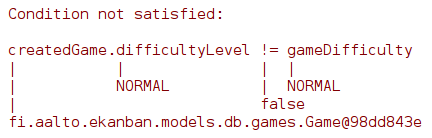
\includegraphics[width=10cm]{images/spock-debug.png}
        \end{topbot}
        \caption{Spock console debugger}
        \label{fig:spock-debug}
      \end{center}
    \end{figure}

    As stated earlier, Spock is a BDD testing framework with Gherkin support.
    Full functionality of Gherkin includes feature and scenario information described
    with \textbf{Given-When-Then} steps for plain text test input~\cite{gherkin}. This makes it easier for stakeholder collaboration
    and is aimed at acceptance testing level.
    Spock supports full Gherkin through additional library \textit{Pease}, but the support for it is deprecated~\cite{spock-pease}.
    Although Spock can be configured to use plain text Gherkin, its normal usage is aimed for developer audience at implementation
    level with test code and Gherkin descriptions mixed in together~\cite{okolnychyi2016study}.

    \begin{figure}[ht]
        \begin{lstlisting}[style=java]
    class GameServiceSpockSpec extends Specification {

        %%@Shared%% GameService gameService
        %%@Shared%% GameInitService gameInitService
        %%@Shared%% GameRepository gameRepository

        <<def>> setup() {
            gameInitService = Mock(GameInitService)
            gameRepository = Mock(GameRepository)
            <<def>> playerService = Mock(PlayerService)
            <<def>> gameOptionService = Mock(GameOptionService)
            gameService = new GameService(gameInitService, playerService,
                                          gameOptionService, gameRepository)
        }
        \end{lstlisting}
        \caption{Spock specification file initialization}
        \label{fig:spock-init}
    \end{figure}

    Spock terminology consists of \textbf{specification} files containing \textbf{feature methods} and Given-When-Then
    \textbf{blocks} inside them~\cite{spock}. Figure \ref{fig:spock-init} displays initialization of a Spock specification
    file. At line \#1 the specification class is created by extending the class \textit{Spock.lang.Specification}. Lines
    3-5 show use of \textit{@Shared}-variables, which are used for long lived objects shared between feature methods~\cite{spock}.
    Lines 7 to 14 show the use of \textit{setup}-fixture for creating a shared, isolated context for each feature method~\cite{spock}.
    The fixture setup is used for initializing unit testing context, where the use of \textit{Mock}-objects~\cite{spock} can be seen.
    Class under test \textit{GameService} has its dependencies replaced with test doubles.

    Spock makes heavy use of Gherkin's Given-When-Then with runnable code blocks for each steps, that can contain textual
    description~\cite{kapelonis2016java}:
    \begin{itemize}
    \item \textbf{Given} is a code block used to initialize the \textbf{context} of test
    \item \textbf{When} is a code block used to trigger the \textbf{action}, stimulus of the test
    \item \textbf{Then} is a code block containing assertions to verify \textbf{conditions}
    \end{itemize}
    JUnit testing literature also states to use this kind of structure with \textbf{Arrange-Act-Assert (AAA)},
    where different parts are separated from each other with space between them~\cite{langr2015pragmatic}.
    As this structure is not enforced in JUnit, there is the considerable possibility that it will not be used~\cite{kapelonis2016java}.

    Figure \ref{fig:spock-example} illustrates the contents of a feature method and the use of Given-When-Then blocks.
    Block definitions are at lines 4, 10, 13, 17, 20 and 23 together
    with optional~\cite{spock} textual descriptions.
    Lines 4-8 form a \textit{Setup}-block, which is an alias for Given-block~\cite{spock}.
    Lines 17 and 20 display the creating of \textit{And}-block, which can be used as
    an alias for the previously occurred main block (Given-When-Then) for more readable structure~\cite{kapelonis2016java}.

    \clearpage
    \begin{figure}[H]
        \begin{lstlisting}[style=java]
    $$@Unroll
    <<def>> "GameService startGame() with playerName #playerName and difficulty #gameDifficulty"() {

        !!setup:!!
            <<def>> newGame = GameBuilder.aGame()
                            .withPlayerName(playerName)
                            .withDifficultyLevel(gameDifficulty)
                            .build()

        !!when:!! "startGame() is called with playerName and gameDifficulty"
            <<def>> createdGame = gameService.startGame(playerName, gameDifficulty)

        !!then:!! "game should be initialized and persisted"
            1 * gameInitService.getInitializedGame(gameDifficulty, playerName) >> newGame
            1 * gameRepository.save(newGame) >> newGame

        !!and:!! "game has been created with given name"
            createdGame.playerName == playerName

        !!and:!! "game has been created with given gameDifficulty"
            createdGame.difficultyLevel != gameDifficulty

        !!where:!!
            playerName | gameDifficulty
            "Player"    | GameDifficulty.NORMAL
            "Pelaaja"   | GameDifficulty.NORMAL

    }
          \end{lstlisting}
        \caption{Spock feature method}
        \label{fig:spock-example}

    \end{figure}
    Lines 14-15 display the verifying of mock object actions and stubbing capabilities.
    For example, at line 14
    \begin{center}
    \textit{1 * gameInitService.getInitializedGame(gameDifficulty, playerName)}
    \end{center}
    verifies that the mock object method is called exactly one time with exact defined parameters \textit{gameDifficulty} and \textit{playerName}.
    The latter part after the verifying, \textit{"\textgreater\textgreater} \textit{newGame"}, is used to stub the return value for the
    called mock object action.

    DDT can be seen with lines 1 and 23-26.
    Line 1 \textit{@Unroll} creates a separate test run for each parameter
    variation defined in the \textit{Where}-block (lines 23-26). Line 24. defines the parameter names and lines 25-26 are
    separate situations that creates an individual feature method run. Finally the line 27. holds the definition of
    the feature method. The name of feature method can be inserted as a string description, allowing more easily to write
    information in it~\cite{kapelonis2016java}. In the example, name holds test run output information with the embedded parameters inside it.
    The result of feature method run on the IDE Intellij Idea can be seen in the figure \ref{fig:spock-result} as two separate test runs through the DDT.

    To get Spock integrated into \textit{Gradle} build cycle with full mocking capabilities, Spring Framework support and BDD styled HTML-reporting, it needs
    quite a few dependencies. The build configuration can be found in Appendix \ref{chapter:gradle-build} figure \ref{fig:spock-build}.

    \clearpage
    \begin{figure}[H]
      \begin{center}
        \begin{topbot}[style=mdstyle]
        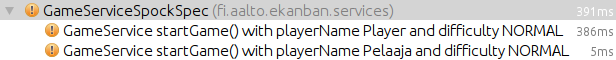
\includegraphics[width=\textwidth]{images/spock-result.png}
        \end{topbot}
        \caption{Spock feature method output}
        \label{fig:spock-result}
      \end{center}
    \end{figure}
    All the examples displayed in the figures are of Spock used for testing Java-code. Although at first glance the test code might
    look like Java, the programming language used is Groovy. Groovy is aimed to resemble Java with dynamic programming language
    capabilities and less verbose syntax~\cite{kapelonis2016java}. In the given test code examples, Java production code classes are used directly
    from Groovy.

    Next chapter explains the research around testing Java-code with different testing possibilities explained in this environment
    chapter. Chapter \ref{chapter:methods} will first explain what the empicical research focuses on and then how it does it.

